\chapter{サンプル章}
\label{ch:introduction}

この章は、テンプレートの各機能の使い方を示すサンプルです。
実際の執筆ではこのファイルを書き換えるか、コピーして章を増やしてください。

\section{数式マクロと定理環境}

プリアンブルで定義済みのマクロは、たとえば集合 $\CC$, $\RR$, $\ZZ$ や
ブラケット記法 $\ket{\psi}$, $\bra{\phi}$, $\braket{\phi}{\psi}$ のように使えます。

\begin{definition}\label{def:sample}
サンプルの定義です。ここに定義本文を書きます。
\end{definition}

\begin{theorem}\label{thm:sample}
サンプルの定理です。定義\ref{def:sample}を用いて主張を述べます。
\end{theorem}
\begin{proof}
ここに証明を書きます。
\end{proof}

\section{図}

図を挿入するには、外部の画像ファイルを使う場合は
\verb|figures/introduction/| のように章と同名のディレクトリに置き、
\verb|\includegraphics{introduction/ファイル名}| として呼び出します
（\verb|\graphicspath| により \verb|figures/| が探索対象になっています）。

数式的な図を直書きしたい場合は、以下のように \texttt{tikzpicture} を使えます。

\begin{figure}[htbp]
  \centering
  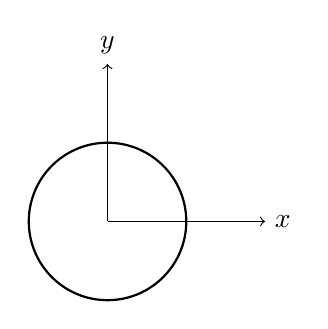
\begin{tikzpicture}
    \draw[->] (0,0) -- (2,0) node[right] {$x$};
    \draw[->] (0,0) -- (0,2) node[above] {$y$};
    \draw[thick] (0,0) circle (1);
  \end{tikzpicture}
  \caption{TikZによるサンプル図}
  \label{fig:sample}
\end{figure}

図\ref{fig:sample}のように、単位円を描いています。

\section{参考文献と索引}

参考文献は \verb|bibliography/references.bib| に追記し、
\verb|\cite{}| で引用します。たとえば\cite{sample:book}や\cite{sample:article}のように
使います。

索引に載せたい用語には \verb|\index{}| を使います\index{索引の使い方}。
索引\index{さくいん@索引}や定理\index{ていり@定理環境}といった見出し語を
このように埋め込むと、巻末の索引に自動的に集約されます。
